\chapter{Detailed design}

\section{Actor model}

\section{Rooms}

\subsection{ServerRoom}
\begin{figure}[h]
	\centering
	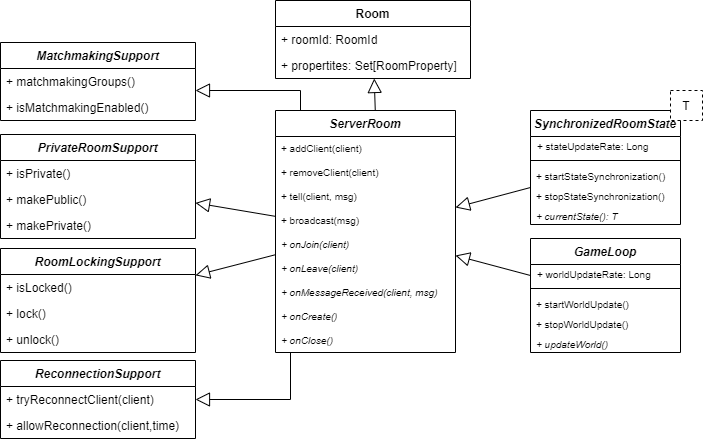
\includegraphics[scale=0.6]{images/4-design/server-room.png}
	\caption{Server room class diagram}
	\label{fig:server_room_class_diagram}
\end{figure}

\subsection{ClientRoom}

\subsection{Properties and Filters}

\section{Server}

\section{Client}

\section{Communication}\label{sec:communication_design}


\subsection{Json Serialization}
For Request-Response interaction (described in section 3.4), we decided to use json format for both client requests and server responses. We have defined a class that provides json-formatted serialization capabilities for all entities that are exchanged at this stage of client-server interaction that are specifically:
\begin{itemize}
	\item SharedRoom objects
	\item Room properties
	\item Room filters
\end{itemize}

\subsection{Websockets}
\begin{figure}[]
	\hspace*{-0.5in}
	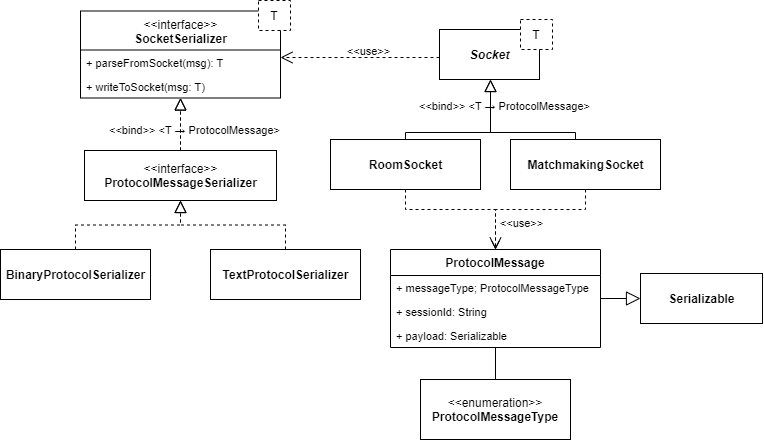
\includegraphics[scale=0.6]{images/4-design/communication_protocol.png}
	\caption{Websocket class diagram}
	\label{fig:websocket_communication_design}
\end{figure}
Regarding websockets instead, the design is more structured. A class diagram describing the main classes is shown in figure \ref{fig:websocket_communication_design}.
The \texttt{Socket} abstract class provides the main functionalities for a socket communication and allows to define the configurations for the connection: heartbeat rate and idle timeout. It is generic in T where T represents the type of messages sent through that socket . Two concrete implementations are provided for this class:
\begin{itemize}
	\item \texttt{RoomSocket}: used for the communication between client and rooms.
	\item \texttt{MatchmakingSocket}: used for the communication between client and matchmaking servicess
\end{itemize}
They both are Socket where the generic type T is a \texttt{ProtocolMessage}. This is indeed the class that defines the communication protocol between client and server. It has 3 fields to describe a message sent through a socket:
\begin{itemize}
	\item \textit{messageType} \\
	Used to identify the type of message that the client or the server want to send. The list of the possible message types is defined in the ProtocolMessageType enumeration.
	\item \textit{sessionId} \\
	This is used to identify the client that is sending the message through the socket. When a websocket connection is established between client and server, a unique id is genereated; the client must always uses the same sessionId to send messages through that socket.
	\item \textit{payload} \\ 
	An optional payload that can be carried with the massage. This is for example the field that is set when the developer use the 'sendMessage' method on the client room. It must be Serializable since it will eventually be serialized to be sent to the server.
\end{itemize}

In order for a Socket object to send and receive data, it must be able to serialize and deserialize the messages that pass through it. It uses for this purpose a \texttt{SocketSerializer} that has two methods: parsefromSocket and writeToSocket. This class is also generic in T that is the type of messages that needs to read and write.

Since \texttt{RoomSocket} and \texttt{MatchmakingSocket} needs to handle \texttt{ProtocolMessage}s we defined a \texttt{ProtocolMessageSerializer} interface that specifically defines a serializer for protocol messages. We implemented two types of serializers: \texttt{BinaryProtoclSerializer} and \texttt{TextProtocolSerializer}. The first one serialize protocol messages as binary data; the latter instead as text messages.
 
We have two different implementations because we initially thought to use json also for socket communication and this would be done by the \texttt{TextProtocolSerializer}. However we eventually decided to use binary representation both to improve performance and usability, so we switched to the \texttt{BinaryProtoclSerializer}


An example of a full interaction between client and server is shown in the sequence diagram in figure \ref{fig:create_room_seq}
\begin{figure}[]
	\hspace*{-1in}
	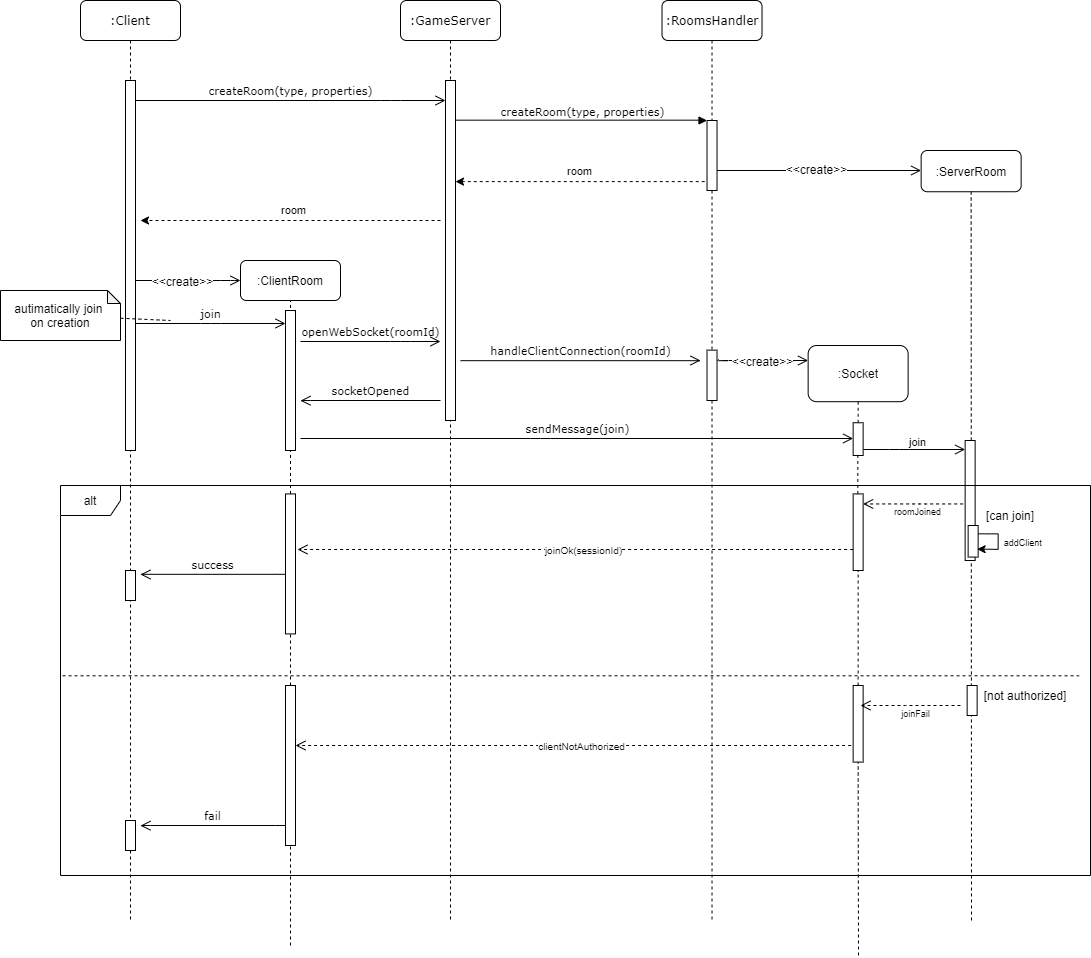
\includegraphics[scale=0.5]{images/4-design/crate_room_seq.png}
	\caption{Example of a client-server interaction upon a 'create room' request}
	\label{fig:create_room_seq}
\end{figure}